\documentclass[class=book, crop=false]{standalone}
\usepackage[subpreambles=true]{standalone}

\usepackage{../../style}

\graphicspath{{./assets/images/}}

\begin{document}
\chapter{L'architettura MIPS}

Dopo la breve introduzione del precedente capitolo, affronteremo ora lo studio dell'architettura \textit{MIPS}; iniziamo con questa perché, seppur non molto diffusa, è molto simile ad altre architetture che vedremo in seguito (soprattutto ARM), ed è quindi prodepeutica.

\section{Breve riepilogo su ISA}
Come sappiamo già, ogni processore possiede un proprio linguaggio macchina, che non è altro che una sorta di "vocabolario di istruzioni" detto \emph{Instruction Set Architecture} (o \emph{ISA} per gli amici); queste istruzioni sono solitamente le operazioni aritmetiche fondamentali (a parte quelle che lavorano su floating point) e quelle logiche. \\
Nonostante ogni processore possieda un proprio ISA, le differenze non sono poi così grandi (motivo per cui conoscere MIPS ci agevolerà molto nell'appren-dimento di altre ISA); una similitudine adeguata può essere fatta con i dialetti di una lingua maggiore (per esempio, veneziano, trevigiano e veronese sono tutte varianti locali mutualmente intelligibili della Grande Lingua Veneta).\\
Lo scopo di avere questi sistemi di istruzioni è poter controllare e sfruttare la potenza di calcolo fornita dai nostri calcolatori; inoltre, come già fatto notare da Von Neumann nel 1947, la progettazione di un'architettura influisce enormemente sull'efficienza dell'hardware, ed è fondamentale che si ricerchino istruzioni \emph{semplici, chiare e veloci}.\\
Un organico di istruzioni andrà a costruire un \emph{programma memorizzato} che, come approfondiremo, altro non è che un insieme di istruzioni che, come numeri e qualsiasi altro dato, andrà mappato sotto formadi numero binario.

\subsubsection{Cos'è MIPS}
Come già detto, nonostante non sia diffusissima, inizieremo a studiare l'architettura MIPS in quanto propedeutica. È una cosiddetta architettura RISC "pragmatica", ossia un'architettura ibrida che, pur essendo basata su RISC e quindi con un numero limitato di istruzioni disponibili, possiede anche alcune operazioni complesse tipiche delle ISA CISC.\\
Fin dai tempi di Von Neumann era chiaro che, per quanto semplice e vicino al linguaggio macchina un linguaggio potesse essere, non dovevano mancare le operazioni aritmetiche e logiche fondamentali; oltre a quelle, MIPS possiede inoltre alcuni comandi per il controllo di flusso.

\section{Operazioni aritmetiche}
Per dare una chiave di lettura al percorso che faremo su MIPS useremo alcuni principi di progettazione software e hardware che ogni informatico segue fin dagli albori della storia dell'informatica, e naturalmente, iniziando a parlare delle operazioni aritmetiche,  inizieremo così:\\

\textbf{PRINCIPIO DI PROGETTAZIONE N. 1:}\\
\emph{La semplicità favorisce la regolarità}.\\

In linea con questo principio, MIPS consente di effettuare operazioni aritmetiche solo nella loro forma più semplice, ossia con tre operandi: \(a = b + c\).
Quest'istruzione, comune in C, Java, Python o altri linguaggi, in MIPS sarà scritta così:
\begin{minted}{asm}
	add a, b, c;
\end{minted}

Notiamo subito che l'operando "di destinazione" viene messo come primo elemento (in altre ISA non è sempre così, tuttavia).\\
Naturalmente, mentre nei linguaggi ad alto livello possiamo agevolmente scrivere espressioni matematiche complesse, in MIPS verranno tutte mappate in espressioni semplici, sicché una linea di codice, per quanto semplice
\begin{minted}{c}
	f = (g + h) - (i + j);
\end{minted}
può essere srotolata in molte righe assembly.
\begin{minted}[linenos]{asm}
	add t0, g, h;  # t0 (variabile temp) = g + h
	add t1, i, j;  # t1 (variabile temp) = i + j
	sub f, t0, t1;  # f = t0 - t1
\end{minted}
Notiamo inoltre che i commenti si scrivono con \#, e questo agisce solo sulla riga (anche se, come detto prima, non sempr è così; ad esempio GCC, l'assembler di Unix, usa i commenti come il C e l'operando di destinazione va in fondo).

\section{I registri}

\subsection{Cosa sono}

Fino ad ora abbiamo considerato gli operandi come fossero normali variabili, ma in realtà questi altro non sono che dei \emph{registri}, ossia delle particolari locazioni di memoria interne al processore e che possono essere reperite celerissimamente, con un solo colpo di clock.\\
MIPS possiede 32 registri, ciascuno di 32 bit, per cui ogniqualvolta si debba eseguire delle operazioni è necessario caricare i dati dalla RAM con un'operazione di \emph{load}. Questo processo può apparire dispendioso ed è lecito domandarsi come mai non ci si possa dotare di più registri più capienti, e la risposta è espressa dal\\

\textbf{PRINCIPIO DI PROGETTAZIONE N.2:}\\
\emph{Minori dimensioni portano a maggiore velocità}\\

Di fatto, se avessimo  più registri, aumenterebbe notevolmente il tempo di accesso a questi, in quanto gli impulsi elettrici impiegherebbero fisicamente più tempo per passare da un registro all'altro, e la velocità di clock sarebbe visibilmente compromessa.

\subsection{Gestione dei registri}

\paragraph{Notazione}
A questo punto, tornando all'esempio di prima, illustriamo la sintassi per richiamare un registro:
\begin{minted}[linenos, breaklines]{asm}
	add $t0, $s1, $s2;  # al registro temporaneo t0 viene assegnato il valore come somma di s1 + s2
	add $t1, $s3, $s4;  # same as before
	sub $s0, $t0, $t1;  # f = t0 - t1
\end{minted}
Come si evince, è sufficiente anteporre un \$ al nome del registro.
\subsubsection{Movimenti}Naturalmente, i registri non sono minimamente sufficienti per contenere tutte i dati di un programma complesso (soprattutto perché alcuni vengono usati dal kernel e dal sistema operativo), ma le operazioni possono essere eseguite solo fra registri. Diventa quindi necessaria l'implementazione delle funzioni \emph{load} che, come anticipato, carica i dati dalla RAM a un registro, e \emph{store}, che passa il dato dal registro alla RAM.\\
La memoria è solitamente organizzata in gruppi da 8 bit, ma il prelievo e il salvataggio dei dati segue un cosiddetto \textbf{vincolo di allineamento}: viene fissato un \emph{offset (spiazzamento)} di 4 byte (quindi della stessa dimensione dei registri), dimodoché ogni informazione che passa abbia la medesima dimensione di un registro (anche il program counter viene incrementato di 4 byte ogni fetch); in questo contesto, ogni informazione di 4 byte che viene spostata tra RAM e registri viene detta \emph{parola}.\\
L'indirizzo di ogni parola viene quindi espresso con una \emph{base}, specifica per registro, e con lo \emph{spiazzamento} costante di cui abbiamo parlato prima.

\paragraph{Load and store}
Ecco un esempio di istruzione di load (analogamente per la store):
\begin{figure}[H]
	\centering
	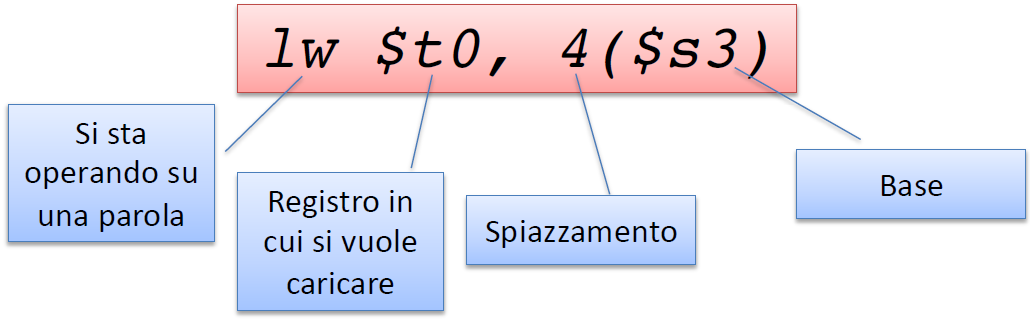
\includegraphics[width=0.7\textwidth,keepaspectratio]{load}
	\caption{Descrizione di una \emph{load}}
\end{figure}
Adesso prendiamo invece una semplice riga di codice:
\begin{minted}{c}
	A[12] = h + A[8];
\end{minted}
E vediamone ora la traduzione fatta dal compilatore:
\begin{minted}[linenos, breaklines]{asm}
	lw $t0, 32($s3);   # la parola 8 comincia all'indirizzo 32 e il puntatore A è in $s3
	add $t0, $s2, $t0; # h è in $s2
	sw $t0, 48($s3);   # memorizzo il contenuto di $t0 in A[12]
\end{minted}
Questo è un esempio un po' più complesso, si raccomanda una lettura accorta per comprendere ogni azione.

\paragraph{Register Spiling}
Come già anticipato, i 32 registri non sono assolutamente sufficienti per contenere tutte le variabili usate da un programma complesso, quindi quello che succede a livello assembly è un continuo susseguirsi di load e store, e questa operazione si chiama \emph{register spilling} ed è eseguita dal compilatore (si dice che  prepara il \emph{working set} e stima le load e store appropriate).

\subsection{Le costanti}
Molto spesso ci si trova a lavorare con le costanti. Nonostante ogni costante possa essere salvata su un registro, questa soluzione è parecchio inefficiente, perché le costante e le operazioni relative sono molto comuni.\\

\textbf{PRINCIPIO DI PROGETTAZIONE N.3:}\\
\emph{Rendi veloci le operazioni comuni}.\\

Quindi ci conviene assolutamente costruire una sintassi dedicata all'esecuzione di operazioni con costanti, dove la \emph{i} sta per \emph{immediate}. Ad esempio:
\begin{minted}{c}
	f = f + 4;
\end{minted}
diventerà
\begin{minted}{asm}
	addi $s3, $s3, 4
\end{minted}

Per dare un altro esempio, è molto conveniente implementare un registro zero (\emph{\$zero}), perché rende molto più semplici le operazioni di copia, che di fatto possono essere ridotte a una somma di un qualsiasi registro con il registro zero.
\section{La rappresentazione delle istruzioni}

\subsubsection{Convenzioni sulla scrittura esadecimale}
Prima di indicare come vengono codificate le istruzioni, ricordiamo che 1 byte è agevolmente rappresentabile con due cifre esadecimali (essendo composto da 8 bit e sapendo che ogni cifra esadecimale corrisponde a 4 bit). Ad esempio, \(1001 1101_{2}\) diventa \(9D_{16}\). Inoltre, quando scriviamo in esadecimale, si usa di solito precedere la scrittura con \emph{0x}. Esempio: \emph{0xEA01BD1C}.\\
Quando si devono codificare parole di 4 byte è importante decidere dove va il byte più significativo.
\begin{itemize}[nolistsep]
	\item Se il byte più significativo è posto per primo, la notazione è detta \emph{little endian} (usata nei processori Motorola e protocolli internet).
	\item Se il byte più significativo è posto per primo, la notazione è detta \emph{big endian} (usata nei processori Intel).
\end{itemize}

\subsection{Le istruzioni in MIPS}
Come anticipato, le istruzioni vengono mappate come numeri binari. In particolare, ogni istruzione dovrà essere mappata utilizzando parole di soli 32 bit, ma come viene impostato questo processo?\\
% TODO - capire per quale motivo non funzioni \mintinline{asm}{...}
Prendiamo come esempio l'istruzione di somma \mintinline{asm}{add \$t0, $s1, $s2}: avremo bisogno di un codice per l'istruzione di somma e uno per ogni registro; l'operazione sarà scritta nei primi 6 bit e negli ultimi 6, mentre i 20 in bit in mezzosaranno divisi in gruppi da 5 bit ciascuno, e i primi tre gruppi ospiteranno i registri, e l'ultimo sarà usato per comandi speciali (come lo shift, che vedremo in seguito).
\begin{figure}[H]
	\centering
	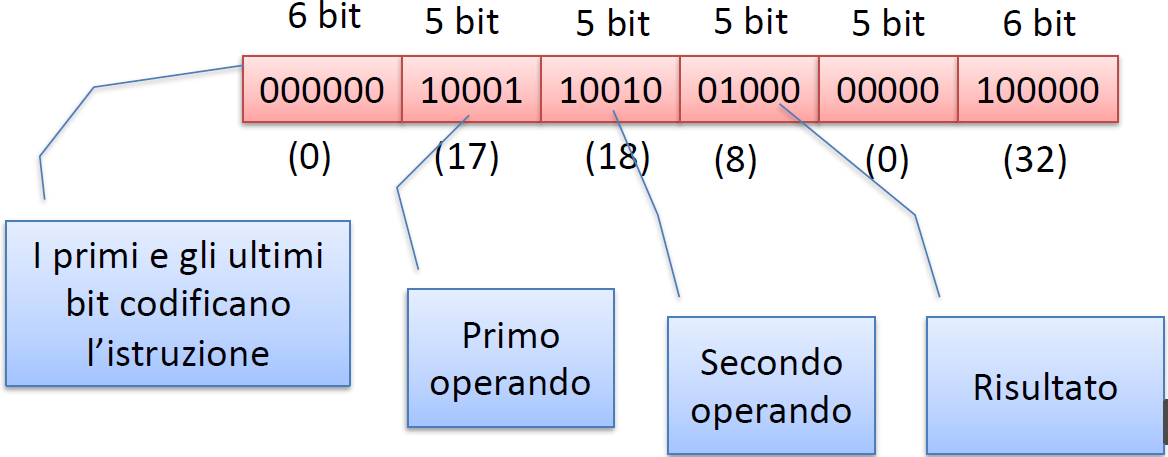
\includegraphics[width=0.8\textwidth,keepaspectratio]{istruzioni.png}
	\caption{Esempio di somma}
\end{figure}
In gerale questo sistema, detto R (da Registro), ogni campo dell'istruzione ha un nome:
\begin{figure}[H]
	\centering
	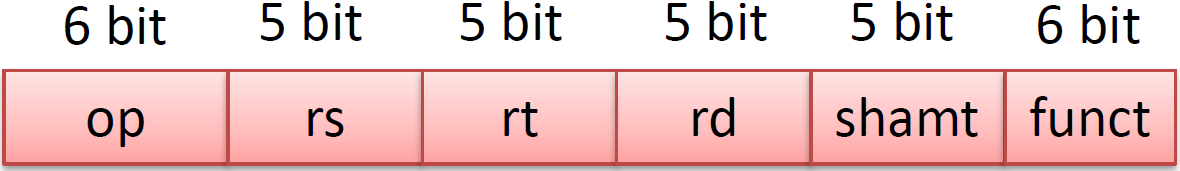
\includegraphics[width=0.9\textwidth,keepaspectratio]{mappatura.png}
	\caption{Mappatura di un'istruzione di tipo R}
\end{figure}
A questo punto è lecito domandarsi come mai si usino solo 32 bit per rappresentare le istruzioni, e la risposta sta nel:\\

\textbf{PRINCIPIO DI PROGETTAZIONE N.4:}\\
\emph{Buoni progetti richiedono buoni compromessi}\\

Uilizzare una quantità limitata di registri e istruzioni e limitandone le dimensioni possiamo guadagnare moltissimo in efficienza!

\subsection{Istruzioni immediate}
Nei casi di indirizzamento immediato e di operazioni con costanti MIPS mette a disposizione una diversa mappatura, detta appunto I. Forniamo qui un esempio e invitiamo il lettore a confrontare la seguente mappatura con l'equivalente R.
\begin{figure}[H]
	\centering
	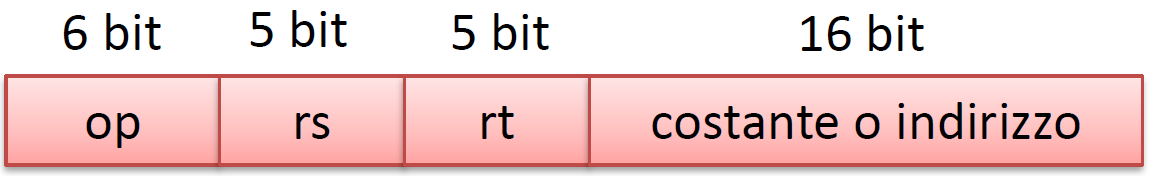
\includegraphics[width=0.7\textwidth,keepaspectratio]{I.png}
	\caption{Mappatura di un'istruzione I}
\end{figure}

esempio immediate?

\section{Istruzioni aritmetico-logiche}

\subsection{Operazioni di shift}

\paragraph{Shift logico a sinistra}
Consideriamo lo \emph{shift logico a sinistra}: l'idea consiste nell'inserire degli zeri nella posizione meno significativa e traslare tutto a sinistra perdendo, nel caso di overflow, i bit più significativi.

\begin{minted}[breaklines]{asm}
ssl $t2, $s0, 4  # memorizza in t2 il contenuto del registro s0 shiftato a sinistra di 4
\end{minted}

Lo shift massimo che è possibile eseguire è di 32 bit (infatti, come precedentemente visto, vengono allocati 5 bit per il campo di \emph{shift amount}). Ciò non risulta un problema in quanto il vincolo di allineamento definito dall'implementazione \emph{MIPS} che affronteremo è costituito da 32 bit.\\
Eseguire uno shift a sinistra di \(k\) bit di un numero \(n\) positivo, consiste nel moltiplicare \(n\) per \(2^k\). Fanno eccezione solo alcuni casi in cui si lavora con numeri interi codificati in complemento a 2: in questo frangente, si potrebbe uscire dal \emph{range di rappresentazione} del CA2.

\paragraph{Shift logico a destra}
In maniera analoga, lo \emph{shift logico a destra} consiste nell'inserire degli zeri nella posizione più significativa, traslando tutto a destra. Come per lo shift logico a sinistra, anche qui è possibile effettuare uno shift di al massimo 32 bit.

\begin{minted}[breaklines]{asm}
srl $t2, $s0, 1  # memorizza in t2 il contenuto del registro s0 shiftato logicamente a destra di 1
\end{minted}

Applicare uno shift logico a destra di \(k\) bit ad un numero \(n\) positivo è equivalente a dividere (divisione intera) \(n\) per \(2^k\). Lo shift logico a destra non è utilizzabile in nessun caso con un numero negativo codificato in CA2 (proprio per questo è stato introdotto lo shift aritmetico a destra).

\paragraph{Shift aritmetico a destra}
Dunque, per trovare una soluzione all'implementazione della divisione intera anche per i numeri negativi codificati in CA2, è stato introdotto lo \emph{shift aritmetico a destra}.

\begin{minted}[breaklines]{asm}
sra $t2, $s0, 1  # memorizza in t2 il contenuto del registro s0 shiftato aritmeticamente a destra di 1
\end{minted}

Piuttosto che inserire 0 come bit più significativo, come avviene nello shift logico, lo shift aritmetico a destra inserisce bit uguali al bit di segno. Dunque risolve i problemi con CA2.\\
Si noti come non abbia senso parlare di shift aritmetico a sinistra, in quanto o il risultato è rappresentabile (attraverso lo shift logico) o non lo è.

\subsection{Operazione di bitwise}
Vengono definite di \emph{Bitwise} quelle operazioni logiche che operano su ciascun bit.
\paragraph{Bitwise AND}
L'operazione di \emph{bitwise AND} viene applicata principlamente per forzare alcuni bit a 0 usando come operando una maschera (i cui bit corrispondenti a quelli che si vogliono annullare sono settati a 0).
\begin{figure}[H]
	\centering
	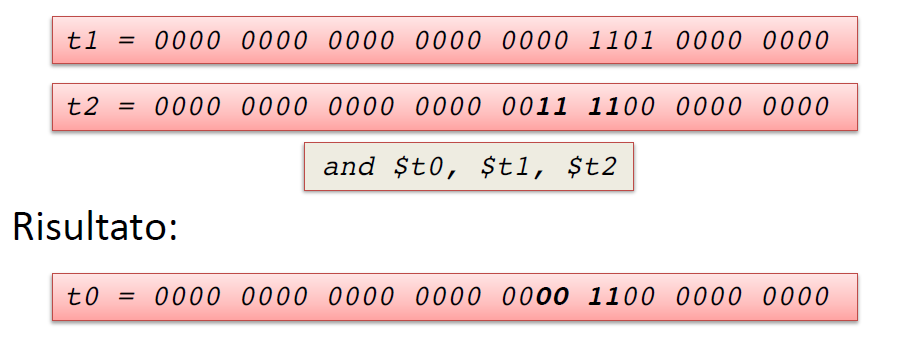
\includegraphics[width=0.7\textwidth,keepaspectratio]{bitwise_and}
	\caption{Funzione "maschera" del bitwise AND}
\end{figure}

\paragraph{Bitwise OR}
In maniera analoga, è possibile settare a \(1\) alcuni bit applicando l'operazione di \emph{bitwise OR} con un operando che abbia \(1\) nella posizione corrispondente (funzione di maschera). Ad esempio, per impostare ad \(1\) i \(4\) bit più significativi di \$s0:
\begin{minted}[linenos, breaklines]{asm}
	addi $t0, $zero, 0x000F
	sll $t0, $t0, 28
	or $s0, $s0, $t0
\end{minted}

Un ulteriore esempio riguarda quello della \emph{rotazione} dei \(4\)bit più significativi di una world sui suoi bit meno significativi:
\begin{minted}[linenos, breaklines]{asm}
	# si ottengono i 4 bit più significativi, spostandoli nei 4 meno significativi di $t0
	srl $t0, $s0, 28

	# si azzerano i 4 bit più significativi di $s0
	sll $s0, $s0, 4
	srl $s0, $s0, 4

	# operazione di maschera
	or $s0, $s0, $t0
\end{minted}

\paragraph{Bitwise NOR}
L'operazione di \emph{NOR} viene definita come segue:
\begin{table}[H]
	\centering
	\subimport{assets/tables/}{nor.tex}
	\caption{Tabella di verità NOR}
\end{table}

A seguire la sintassi MIPS dell'istruzione di \emph{bitwise NOR}:
\begin{minted}[linenos]{asm}
	nor $t0, $t1, $t2
\end{minted}

\paragraph{Bitwise NOT}
Dato il fatto che l'operatore di \emph{NOT} è unario, esso non è implementato in MIPS, per non interrompere la regolarità delle istruzioni a tre operandi. Un modo per ottenere il NOT, grazie alle leggi di De Morgan, è il seguente:
\begin{minted}{asm}
	nor $t0, $t1, $zero  # equivale a: not $s0
\end{minted}

\paragraph{OR esclusivo (XOR)}
L'\emph{OR esclusivo} produce \(1\) se i due bit di ingresso sono uguali, altrimenti \(0\) se sono uguali. Segue la tabella di verità:
\begin{table}[H]
	\centering
	\subimport{assets/tables/}{xor.tex}
	\caption{Tabella di verità XOR}
\end{table}

A seguire la sintassi MIPS dell'operazione di XOR:
\begin{minted}{asm}
	xor $t0, $t1, $t2  # $t0 = $t1 xor $t2
\end{minted}

Curiosità: se si esegue lo XOR di un numero con se stesso, il risultato è pari a \(0\) per ciascun bit.

\section{Salti}
Nella lingua inglese è presente una sostanziale differenza fra \emph{jump} (salto non condizionato) e \emph{branch} (salto condizionato). Il branch modifica il valore del registro \emph{PC}.\\
\begin{minted}{asm}
	beq reg1, reg2, L1; # Branch on EQual
	bne reg1, reg2, L1; # Branch on Non Equal
	j LABEL; salta all'indirizzo di label
	jr $t0; salta all'indirizzo contenuto nel registro
\end{minted}

Le label vengono alla fine tradotte in indirizzi da parte del compilatore.
Il check del branch viene fatto con la condizione opposta, per aver maggiore efficienza.

\subsection{Altri confronti}
\begin{minted}{asm}
	slt $t0, $s3, $s4; # t0=1 se s3<s4
	slti $t0, $s3, 10; # t0=1 se s3<10
\end{minted}

% TODO - Riguarda la parte relativa al segno

\subsection{Implementazione del costrutto \emph{if}}

\subsection{Implementazione del costrutto \emph{while}}
Il ciclo non viene direttamente implementato dal mips.\\
% TODO - Codice C - Codice MIPS (magari affiancati con minipage)

\subsection{Implementazione del costrutto \emph{switch/case}}
\begin{itemize}
	\item Possibilità di creare una sequenza di if-else
	\item
\end{itemize}


\end{document}
